\documentclass[11pt]{article}
\usepackage{amsmath, amssymb, physics, mathtools, bm}
\usepackage{tikz, pgfplots}
\pgfplotsset{compat=1.18}
\usetikzlibrary{calc, positioning}
\usepackage[margin=2.3cm]{geometry}
\usepackage{siunitx, booktabs, hyperref}
\usepackage{braket}

\newcommand{\D}{\mathrm{D}}
\newcommand{\de}{\mathrm{d}}
\newcommand{\pd}[2]{\frac{\partial #1}{\partial #2}}
\newcommand{\pdd}[2]{\frac{\partial^{2} #1}{\partial #2^{2}}}
\newcommand{\Lap}{\nabla^{2}}

\title{B1 Fluids --- Model Solutions, Trinity 2024}
\author{}
\date{}

\begin{document}
\maketitle

\noindent\textit{Throughout, the Navier--Stokes equation for an incompressible viscous fluid under gravity is}
\begin{equation}
\pd{\vb v}{t} + (\vb v \cdot \nabla)\vb v + \frac{1}{\rho}\nabla p + g\hat{\vb z} = \nu \Lap \vb v,
\label{eq:NS}
\end{equation}
\textit{with $\nu$ the kinematic viscosity. We also use $1000~\text{mb}=10^{5}~\text{Pa}$.}

% =====================================================================
\section*{Question 1 --- Stream functions and spin-down of a tank}

\textbf{Problem.} Define streamfunction and vorticity for 2D incompressible flow; verify $\psi=-\Omega(x^2+y^2)/2$ is solid-body rotation. In an elliptical tank $(x/L_x)^2+(y/L_y)^2=1$ with the turntable spinning, sketch laboratory streamlines. After the turntable is halted abruptly (inviscid bulk), find the vorticity, verify $\psi=Ax^2+By^2$, determine $A,B$, sketch streamlines, and discuss paddle-wheel rotation in the bulk and near the wall at high Re.

\subsection*{(a) Stream function, vorticity, and solid body rotation}

For 2D incompressible flow $\vb v=(v_x,v_y,0)$, continuity $\partial_x v_x+\partial_y v_y=0$ admits a streamfunction:
\begin{equation}
v_x = \pd{\psi}{y}, \qquad v_y = -\pd{\psi}{x}.
\label{eq:streamdef}
\end{equation}
$\vb v\cdot\nabla\psi=0$, so $\psi=$ const are streamlines. Vorticity in 2D:
\begin{equation}
\omega = \pd{v_y}{x}-\pd{v_x}{y}.
\label{eq:vortdef}
\end{equation}
Substitute \eqref{eq:streamdef}:
\begin{equation}
\omega = -\Lap\psi.
\label{eq:psivort}
\end{equation}

For $\psi=-\tfrac12\Omega(x^2+y^2)$, differentiate in $y$:
\[ v_x = \pd{\psi}{y} = -\Omega y. \]
Differentiate in $x$:
\[ v_y = -\pd{\psi}{x} = \Omega x. \]
Convert to polars with $x=r\cos\theta$, $y=r\sin\theta$:
\[ \vb v = \Omega r\,\hat{\bm\theta}, \]
i.e.\ rigid rotation at rate $\Omega$. Apply \eqref{eq:psivort}:
\[ \omega = -\Lap\!\left[-\tfrac12\Omega(x^2+y^2)\right]. \]
Evaluate the Laplacian:
\[ \Lap\!\left[-\tfrac12\Omega(x^2+y^2)\right] = -\tfrac12\Omega(2+2) = -2\Omega. \]
Therefore
\begin{equation}
\boxed{\;\omega = 2\Omega.\;}
\end{equation}

\subsection*{(b) Streamlines in the laboratory frame for an elliptical tank}

In the laboratory frame the spun-up fluid rotates rigidly at $\Omega$, so streamlines are concentric circles centred on the tank axis.
\begin{center}
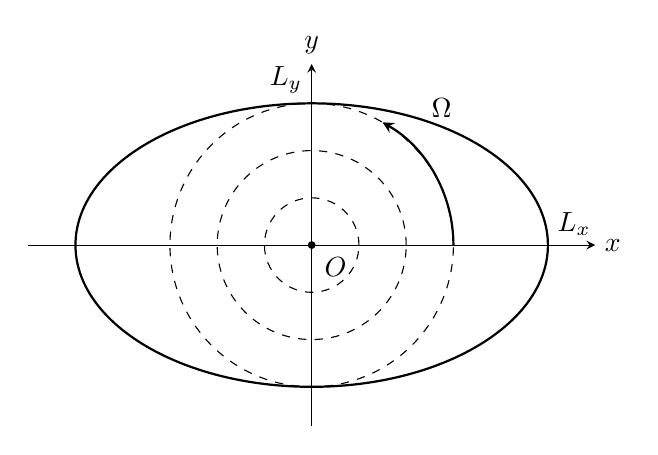
\begin{tikzpicture}[>=stealth, scale=1.0]
  % ellipse
  \draw[thick] (0,0) ellipse (3 and 1.8);
  % concentric circular streamlines
  \foreach \r in {0.6, 1.2, 1.8} {\draw[dashed] (0,0) circle (\r);}
  % axes
  \draw[->] (-3.6,0) -- (3.6,0) node[right] {$x$};
  \draw[->] (0,-2.3) -- (0,2.3) node[above] {$y$};
  % wall labels
  \node[circle,fill,inner sep=1.0pt,label=below right:{$O$}] at (0,0) {};
  \node[above right] at (3,0) {$L_x$};
  \node[above left] at (0,1.8) {$L_y$};
  % rotation arrow
  \draw[->,thick] (1.8,0.0) arc (0:60:1.8);
  \node[above right] at (1.4,1.5) {$\Omega$};
\end{tikzpicture}
\end{center}
The circular streamlines cross the elliptical wall near the major-axis tips ($r\approx L_x$). No fluid actually passes through the wall: the wall is co-rotating, and at each instant it occupies the position the streamline indicates. Steady streamlines coincide with a rigid boundary only in the frame in which that boundary is at rest --- here, the rotating frame, where the fluid is at rest and no streamlines exist.

\subsection*{(c) Vorticity after the turntable is halted; verification of $\psi=Ax^2+By^2$}

Inviscid bulk: Kelvin's theorem freezes vorticity onto fluid elements. Just before stopping, every element had $\omega=2\Omega$; just after,
\begin{equation}
\omega = 2\Omega.
\label{eq:postvort}
\end{equation}

For $\psi=Ax^2+By^2$, differentiate in $y$:
\[ v_x = \pd{\psi}{y} = 2By. \]
Differentiate in $x$:
\[ v_y = -\pd{\psi}{x} = -2Ax. \]
Compute the Laplacian:
\[ \Lap\psi = 2A+2B. \]
Apply \eqref{eq:psivort}:
\[ \omega = -2(A+B). \]
Match with \eqref{eq:postvort}:
\[ -2(A+B) = 2\Omega. \]
Divide by $-2$:
\[ A+B = -\Omega. \tag{i}\label{eq:vortcond}\]
Wall is a streamline, so $\psi=Ax^2+By^2=C$ on $(x/L_x)^2+(y/L_y)^2=1$. The two ellipse equations must define the same curve, so $Ax^2+By^2=C$ is proportional to $x^2/L_x^2+y^2/L_y^2=1$:
\[ A = \frac{C}{L_x^2},\qquad B = \frac{C}{L_y^2}. \tag{ii}\label{eq:wallcond}\]
Substitute \eqref{eq:wallcond} into \eqref{eq:vortcond}:
\[ \frac{C}{L_x^2}+\frac{C}{L_y^2} = -\Omega. \]
Factor $C$:
\[ C\,\frac{L_x^2+L_y^2}{L_x^2 L_y^2} = -\Omega. \]
Solve for $C$:
\[ C = -\frac{\Omega L_x^2 L_y^2}{L_x^2+L_y^2}. \]
Divide by $L_x^2$ for $A$ and by $L_y^2$ for $B$:
\begin{equation}
\boxed{\;A = -\frac{\Omega L_y^2}{L_x^2+L_y^2},\qquad B = -\frac{\Omega L_x^2}{L_x^2+L_y^2}.\;}
\label{eq:ABfinal}
\end{equation}

\subsection*{(d) Streamlines in the spin-down flow and paddle wheel motion}

Streamlines $\psi=$ const are nested ellipses similar to the wall, $(x/L_x)^2+(y/L_y)^2=$ const.
\begin{center}
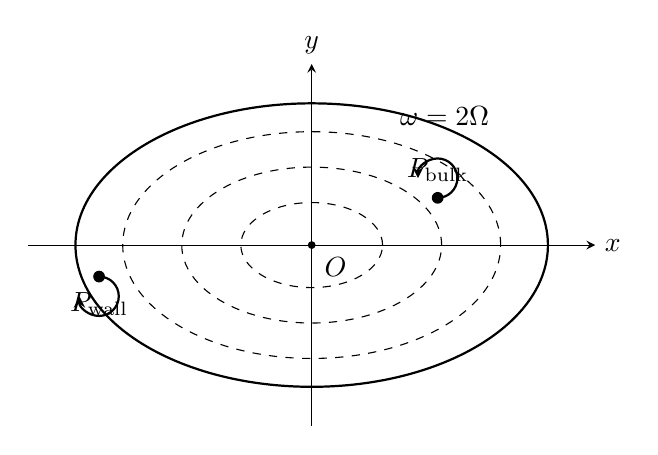
\begin{tikzpicture}[>=stealth, scale=1.0]
  \draw[thick] (0,0) ellipse (3 and 1.8);
  \foreach \s in {0.3, 0.55, 0.8} {\draw[dashed] (0,0) ellipse ({3*\s} and {1.8*\s});}
  \draw[->] (-3.6,0) -- (3.6,0) node[right] {$x$};
  \draw[->] (0,-2.3) -- (0,2.3) node[above] {$y$};
  \node[circle,fill,inner sep=1.0pt,label=below right:{$O$}] at (0,0) {};
  % bulk paddle wheel
  \node[circle,fill,inner sep=1.5pt,label=above:{$P_\text{bulk}$}] (Pb) at (1.6,0.6) {};
  \draw[->,thick] (Pb) ++(0.0,0.0) arc (-90:180:0.25);
  % boundary-layer paddle wheel (near wall)
  \node[circle,fill,inner sep=1.5pt,label=below:{$P_\text{wall}$}] (Pw) at (-2.7,-0.4) {};
  \draw[->,thick] (Pw) ++(0.0,0.0) arc (90:-180:0.25);
  \node[above right] at (1.0,1.4) {$\omega=2\Omega$};
\end{tikzpicture}
\end{center}

Bulk paddle wheel: local vorticity $\omega=2\Omega$ equals twice the local angular velocity, so the wheel spins on its own axis at rate $\Omega$ in the original sense while drifting along an ellipse.

Boundary layer: at high Re viscosity has only diffused a sliver of thickness $\delta\sim\sqrt{\nu t}$ into the wall. No-slip pulls the tangential velocity from its inviscid value down to zero across $\delta$:
\[ \omega_\text{wall} \sim -\frac{v_t}{\delta}, \]
of opposite sign to the bulk $2\Omega$. A wheel sitting in this layer therefore spins counter to one in the bulk.

% =====================================================================
\section*{Question 2 --- Velocity potential, Bernoulli, deep-water surface waves}

\textbf{Problem.} Define the velocity potential, derive Laplace's equation and the unsteady Bernoulli equation. For deep-water waves $\eta=A\cos(kx-\omega t)$, derive the linearised kinematic boundary condition, the dynamic surface BC, solve for $\phi$, derive $\omega=\sqrt{gk}$, compare phase and group speeds; sketch a wave packet. Find $v_x,v_z$ at the surface, sketch the parcel orbit, and state the vorticity.

\subsection*{(a) Potential, Laplace's equation and the Bernoulli relation}

Irrotational flow $\nabla\times\vb v=0$:
\begin{equation}
\vb v = \nabla\phi.
\label{eq:phidef}
\end{equation}
Impose incompressibility $\nabla\cdot\vb v=0$:
\begin{equation}
\Lap\phi = 0.
\label{eq:laplacephi}
\end{equation}

Set $\nu=0$, $\rho=$ const in \eqref{eq:NS}. Apply the vector identity:
\[ (\vb v\cdot\nabla)\vb v = \tfrac12\nabla|\vb v|^2 - \vb v\times(\nabla\times\vb v). \]
Use $\nabla\times\vb v=0$:
\[ (\vb v\cdot\nabla)\vb v = \tfrac12\nabla|\nabla\phi|^2. \]
Substitute \eqref{eq:phidef} into the time derivative:
\[ \pd{\vb v}{t} = \nabla\pd{\phi}{t}. \]
Write $g\hat{\vb z}=\nabla(gz)$. Insert all of these into \eqref{eq:NS}:
\[ \nabla\!\left(\pd{\phi}{t}+\tfrac12|\nabla\phi|^2+\frac{p}{\rho}+gz\right) = 0. \]
Integrate (absorb time-dependent constant into $\phi$):
\begin{equation}
\boxed{\;\pd{\phi}{t}+\frac{|\nabla\phi|^2}{2}+\frac{p}{\rho}+gz = C.\;}
\label{eq:bernoulli}
\end{equation}
Terms: $\partial_t\phi$ unsteady, $\tfrac12|\vb v|^2$ kinetic, $p/\rho$ pressure work, $gz$ gravity. Holds throughout the irrotational fluid at any instant.

\subsection*{(b) Linearised boundary conditions, dispersion relation, group speed}

Kinematic BC: a fluid parcel on the surface stays on the surface, i.e.\ $\D(z-\eta)/\D t = 0$ at $z=\eta$:
\begin{equation}
\pd{\eta}{t} + v_x\pd{\eta}{x} = v_z \qquad \text{at }z=\eta.
\label{eq:KBC-exact}
\end{equation}
Drop the quadratic $v_x\partial_x\eta$ and evaluate at $z=0$:
\begin{equation}
v_z\big|_{z=0} = \pd{\eta}{t}.
\label{eq:KBC-lin}
\end{equation}
Use $v_z=\partial_z\phi$ and differentiate $\eta=A\cos(kx-\omega t)$ in $t$:
\begin{equation}
\pd{\phi}{z}\bigg|_{z=0} = \omega A\sin(kx-\omega t).
\label{eq:KBC-explicit}
\end{equation}

Dynamic BC: pressure on the free surface equals atmospheric (absorb into $C$). Evaluate \eqref{eq:bernoulli} at $z=\eta$:
\[ \pd{\phi}{t}\bigg|_{z=\eta} + \tfrac12|\nabla\phi|^2 + g\eta = 0. \]
Drop the quadratic $\tfrac12|\nabla\phi|^2$ and Taylor-expand $\partial_t\phi$ from $z=\eta$ back to $z=0$ (the correction is $O(\eta\,\partial_z\partial_t\phi)$, second order):
\begin{equation}
\pd{\phi}{t}\bigg|_{z=0} + g\eta = 0.
\label{eq:DBC-lin}
\end{equation}

Deep water: $\phi\to 0$ as $z\to-\infty$. Separate variables, try $\phi = F(z)\sin(kx-\omega t)$. Substitute into $\Lap\phi=0$:
\[ F''(z)\sin(kx-\omega t) - k^2 F(z)\sin(kx-\omega t) = 0. \]
Divide by $\sin(kx-\omega t)$:
\[ F''(z) - k^2 F(z) = 0. \]
General solution: $F=B\mathrm{e}^{kz}+B'\mathrm{e}^{-kz}$. Reject the growing piece by $\phi\to 0$ as $z\to -\infty$:
\[ F(z) = B\,\mathrm{e}^{kz}. \]
Differentiate in $z$ at $z=0$:
\[ \pd{\phi}{z}\bigg|_{z=0} = kB\sin(kx-\omega t). \]
Equate to \eqref{eq:KBC-explicit}:
\[ kB = \omega A. \]
Solve for $B$:
\[ B = \frac{\omega A}{k}. \]
Therefore
\begin{equation}
\phi = \frac{\omega A}{k}\,\mathrm{e}^{kz}\sin(kx-\omega t).
\label{eq:phi-soln}
\end{equation}
Differentiate in $t$ at $z=0$:
\[ \pd{\phi}{t}\bigg|_{z=0} = -\frac{\omega^2 A}{k}\cos(kx-\omega t). \]
Substitute into \eqref{eq:DBC-lin} with $\eta=A\cos(kx-\omega t)$:
\[ -\frac{\omega^2 A}{k}\cos(kx-\omega t) + gA\cos(kx-\omega t) = 0. \]
Divide by $A\cos(kx-\omega t)$:
\[ -\frac{\omega^2}{k} + g = 0. \]
Solve for $\omega^2$:
\[ \omega^2 = gk. \]
\begin{equation}
\boxed{\;\omega = \sqrt{gk}.\;}
\label{eq:disp}
\end{equation}

Compute the phase speed from \eqref{eq:disp}:
\[ c_\text{ph} = \frac{\omega}{k} = \frac{\sqrt{gk}}{k} = \sqrt{\frac{g}{k}}. \]
Differentiate \eqref{eq:disp} to get the group speed:
\[ c_\text{gr} = \dv{\omega}{k} = \tfrac12\,\frac{g}{\sqrt{gk}} = \tfrac12\sqrt{\frac{g}{k}} = \tfrac12 c_\text{ph}. \]

\begin{center}
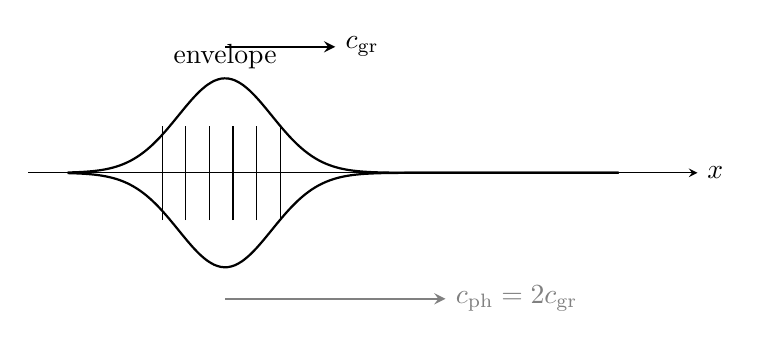
\begin{tikzpicture}[>=stealth, scale=1.0]
  \draw[->] (-0.5,0) -- (8,0) node[right] {$x$};
  % Gaussian envelope at t=0
  \draw[thick,domain=0:7,smooth,samples=80] plot (\x, {1.2*exp(-(\x-2)*(\x-2)/0.7)});
  \draw[thick,domain=0:7,smooth,samples=80] plot (\x, {-1.2*exp(-(\x-2)*(\x-2)/0.7)});
  % carrier ticks inside
  \foreach \x in {1.2,1.5,1.8,2.1,2.4,2.7} {
    \draw (\x,-0.6) -- (\x,0.6);
  }
  % envelope arrow
  \draw[->,thick] (2.0,1.6) -- (3.4,1.6) node[right] {$c_\text{gr}$};
  % phase arrow
  \draw[->,thick,gray] (2.0,-1.6) -- (4.8,-1.6) node[right] {$c_\text{ph}=2c_\text{gr}$};
  \node[above] at (2,1.2) {envelope};
\end{tikzpicture}
\end{center}
A wave packet is a localised superposition; its envelope (and energy) move at $c_\text{gr}$, while individual crests propagate at $c_\text{ph}=2c_\text{gr}$, born at the rear and dying at the front. Deep-water gravity waves are dispersive.

\subsection*{(c) Surface velocity, parcel trajectory and vorticity}

Differentiate \eqref{eq:phi-soln} in $x$ at $z=0$:
\[ v_x = \pd{\phi}{x}\bigg|_{z=0} = \omega A\cos(kx-\omega t). \]
Differentiate in $z$ at $z=0$:
\[ v_z = \pd{\phi}{z}\bigg|_{z=0} = \omega A\sin(kx-\omega t). \]

Linearised Lagrangian trajectory: integrate $\dot x = v_x(x_0,0,t)$ in $t$:
\[ x(t)-x_0 = \omega A\int\cos(kx_0-\omega t)\,\de t = -A\sin(kx_0-\omega t). \]
Integrate $\dot z = v_z(x_0,0,t)$ in $t$:
\[ z(t)-z_0 = \omega A\int\sin(kx_0-\omega t)\,\de t = A\cos(kx_0-\omega t). \]
Square and add, using $\sin^2+\cos^2=1$:
\[ [x-x_0]^2 + [z-z_0]^2 = A^2. \]

\begin{center}
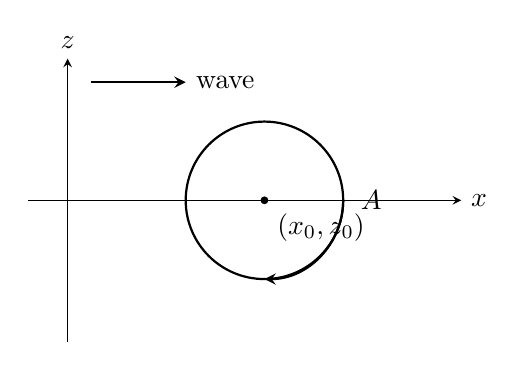
\begin{tikzpicture}[>=stealth, scale=1.0]
  \draw[->] (-0.5,0) -- (5,0) node[right] {$x$};
  \draw[->] (0,-1.8) -- (0,1.8) node[above] {$z$};
  % undisturbed surface (dashed)
  \draw[dashed] (0,0) -- (4.5,0);
  % parcel orbit
  \node[circle,fill,inner sep=1.0pt,label=below right:{$(x_0,z_0)$}] (P) at (2.5,0) {};
  \draw[thick] (P) circle (1.0);
  % rotation sense (clockwise for +x propagation)
  \draw[->,thick] (3.5,0) arc (0:-90:1.0);
  \node[right] at (3.6,0) {$A$};
  % wave propagation arrow
  \draw[->,thick] (0.3,1.5) -- (1.5,1.5) node[right] {wave};
\end{tikzpicture}
\end{center}
Surface parcel moves on a circle of radius $A$, traversed clockwise for $+x$-propagating waves: forward at the crest, downward on the front face, backward in the trough, upward on the rear.

Vorticity in the $(x,z)$-plane: use the full $\vb v=\nabla\phi$ from \eqref{eq:phi-soln}, giving $v_x=\omega A\mathrm{e}^{kz}\cos(kx-\omega t)$ and $v_z=\omega A\mathrm{e}^{kz}\sin(kx-\omega t)$. Differentiate $v_x$ in $z$:
\[ \pd{v_x}{z} = k\omega A\mathrm{e}^{kz}\cos(kx-\omega t). \]
Differentiate $v_z$ in $x$:
\[ \pd{v_z}{x} = k\omega A\mathrm{e}^{kz}\cos(kx-\omega t). \]
Subtract:
\[ \omega_y = \pd{v_x}{z}-\pd{v_z}{x} = 0. \]
\begin{equation}
\boxed{\;\omega_y = 0.\;}
\end{equation}
The flow was assumed irrotational ($\vb v=\nabla\phi$); each parcel orbits without spinning about its own centre.

% =====================================================================
\section*{Question 3 --- Squeeze film between a disk and a table}

\textbf{Problem.} A disk of radius $R$ above a smooth table at $z=0$ is separated by viscous fluid of thickness $h(t)\ll R$, with a small central hole at $r\le a\ll R$. (a) From \eqref{eq:NS} derive the lubrication equation, the no-slip BCs on $v_r$, and show $v_r=-(2\rho\nu)^{-1}\partial_r p\,z(h-z)$. (b) From continuity derive $v_z(z=h)$ and the pressure profile. (c) Compute the lift force for $a=0$, $R=\SI{1}{m}$, $h=\SI{0.5}{mm}$, $\dot h=\SI{1}{mm.s^{-1}}$, $\rho=\SI{e3}{kg.m^{-3}}$, $\nu=\SI{e-6}{m^2.s^{-1}}$, and discuss the effect of a hole.

\subsection*{(a) Thin-film derivation and parabolic velocity profile}

Cylindrical $(r,\theta,z)$, axisymmetric, ignore gravity. Radial component of \eqref{eq:NS}:
\begin{equation}
\pd{v_r}{t}+v_r\pd{v_r}{r}+v_z\pd{v_r}{z}+\frac{1}{\rho}\pd{p}{r} = \nu\!\left[\frac{1}{r}\pd{}{r}\!\left(r\pd{v_r}{r}\right)-\frac{v_r}{r^2}+\pdd{v_r}{z}\right].
\label{eq:NSr}
\end{equation}
Lubrication: $h\ll R$, reduced Reynolds number $\text{Re}\,h^2/R^2\ll 1$. Drop inertia, drop radial viscous terms (smaller by $(h/R)^2$):
\begin{equation}
\frac{1}{\rho}\pd{p}{r} = \nu\,\pdd{v_r}{z}.
\label{eq:thinfilm}
\end{equation}
Vertical momentum gives $\partial_z p=0$, so $p=p(r,t)$.

No-slip at table and disk:
\[ v_r(z=0)=0,\qquad v_r(z=h)=0. \]
Integrate \eqref{eq:thinfilm} once in $z$ (treat $\partial_r p$ as $z$-independent):
\[ \pd{v_r}{z} = \frac{1}{\rho\nu}\pd{p}{r}\,z + C_1(r). \]
Integrate again:
\[ v_r = \frac{1}{2\rho\nu}\pd{p}{r}\,z^2 + C_1(r)z + C_2(r). \]
Apply $v_r(0)=0$:
\[ C_2 = 0. \]
Apply $v_r(h)=0$:
\[ 0 = \frac{1}{2\rho\nu}\pd{p}{r}\,h^2 + C_1\,h. \]
Solve for $C_1$:
\[ C_1 = -\frac{h}{2\rho\nu}\pd{p}{r}. \]
Substitute back and factor:
\[ v_r = \frac{1}{2\rho\nu}\pd{p}{r}(z^2-hz) = -\frac{1}{2\rho\nu}\pd{p}{r}\,z(h-z). \]
\begin{equation}
\boxed{\;v_r = -\frac{1}{2\rho\nu}\pd{p}{r}\,z(h-z).\;}
\label{eq:vrprofile}
\end{equation}

\subsection*{(b) Continuity, vertical velocity and pressure profile}

The relation $r^{-1}\partial_r(rv_r)+\partial_z v_z=0$ is $\nabla\cdot\vb v=0$ in cylindrical coordinates for axisymmetric flow.

Integrate continuity from $z'=0$ (no-slip $v_z=0$ at the table) to $z$:
\[ v_z(r,z,t) = -\int_0^z \frac{1}{r}\pd{}{r}[r v_r]\,\de z'. \]
Substitute \eqref{eq:vrprofile} and pull the $r$-only factor out:
\[ v_z = \frac{1}{2\rho\nu}\,\frac{1}{r}\pd{}{r}\!\left[r\pd{p}{r}\right]\!\int_0^z z'(h-z')\,\de z'. \]
Evaluate the inner integral:
\[ \int_0^z z'(h-z')\,\de z' = \tfrac12 hz^2 - \tfrac13 z^3. \]
Set $z=h$ and simplify $\tfrac12 h\cdot h^2-\tfrac13 h^3$:
\[ \tfrac12 h^3 - \tfrac13 h^3 = \tfrac{1}{6}h^3. \]
Substitute:
\[ v_z(r,h,t) = \frac{h^3}{12\rho\nu}\,\frac{1}{r}\pd{}{r}\!\left(r\pd{p}{r}\right). \]
Match to disk velocity, $v_z(r,h,t)=\dot h$:
\[ \frac{h^3}{12\rho\nu}\,\frac{1}{r}\pd{}{r}\!\left(r\pd{p}{r}\right) = \dot h. \]
Rearrange:
\[ \frac{1}{r}\pd{}{r}\!\left(r\pd{p}{r}\right) = \frac{12\rho\nu\dot h}{h^3}. \]
Multiply by $r$ and integrate in $r$:
\[ r\pd{p}{r} = \frac{6\rho\nu\dot h}{h^3}\,r^2 + C_1. \]
Divide by $r$:
\[ \pd{p}{r} = \frac{6\rho\nu\dot h}{h^3}\,r + \frac{C_1}{r}. \]
Integrate in $r$:
\[ p(r,t) = \frac{3\rho\nu\dot h}{h^3}\,r^2 + C_1\ln r + C_2. \]

Pressure BCs: atmospheric pressure $p_0$ at the outer rim and at the hole (both communicate with the surroundings), $p(R)=p_0$, $p(a)=p_0$:
\[ p_0 = \frac{3\rho\nu\dot h}{h^3}R^2 + C_1\ln R + C_2. \]
\[ p_0 = \frac{3\rho\nu\dot h}{h^3}a^2 + C_1\ln a + C_2. \]
Subtract the second from the first:
\[ 0 = \frac{3\rho\nu\dot h}{h^3}(R^2-a^2) + C_1\ln(R/a). \]
Solve for $C_1$ and flip the sign of the log:
\[ C_1 = -\frac{3\rho\nu\dot h}{h^3}\,\frac{R^2-a^2}{\ln(R/a)} = \frac{3\rho\nu\dot h}{h^3}\,\frac{R^2-a^2}{\ln(a/R)}. \]
Solve the first BC equation for $C_2$:
\[ C_2 = p_0 - \frac{3\rho\nu\dot h}{h^3}R^2 - C_1\ln R. \]
Substitute $C_1,C_2$ back into $p$ and gather:
\[ p = p_0 - \frac{3\rho\nu\dot h}{h^3}(R^2-r^2) + C_1\ln(r/R). \]
Insert the expression for $C_1$:
\begin{equation}
\boxed{\;p(r,t) = p_0 - \frac{3\rho\nu}{h^3}\!\left[(R^2-r^2)-(R^2-a^2)\,\frac{\ln(r/R)}{\ln(a/R)}\right]\dot h.\;}
\label{eq:p-final}
\end{equation}

\subsection*{(c) Lift force and effect of a hole}

For $\dot h>0$, $p<p_0$ throughout the film: atmospheric pressure on the top of the disk exceeds the film pressure below, so the fluid sucks the disk down and a lift force is needed.

Net upward fluid force:
\[ F = \int_a^R [p_0 - p(r,t)]\,2\pi r\,\de r. \]
Set $a=0$: $\ln(a/R)\to -\infty$ while $R^2-a^2\to R^2$, so $(R^2-a^2)\ln(r/R)/\ln(a/R)\to 0$:
\[ p_0 - p(r,t) = \frac{3\rho\nu\dot h}{h^3}(R^2-r^2). \]
Substitute into the force integral:
\[ F = \frac{3\rho\nu\dot h}{h^3}\int_0^R (R^2-r^2)\,2\pi r\,\de r = \frac{6\pi\rho\nu\dot h}{h^3}\int_0^R (R^2-r^2)r\,\de r. \]
Evaluate the integral:
\[ \int_0^R (R^2-r^2)r\,\de r = \frac{R^4}{2}-\frac{R^4}{4} = \frac{R^4}{4}. \]
Multiply:
\begin{equation}
F = \frac{6\pi\rho\nu\dot h}{h^3}\cdot\frac{R^4}{4} = \frac{3\pi\rho\nu\dot h R^4}{2h^3}.
\label{eq:Fnohole}
\end{equation}

Compute the dynamic viscosity:
\[ \mu = \rho\nu = \SI{e3}{kg.m^{-3}}\times\SI{e-6}{m^2.s^{-1}} = \SI{e-3}{Pa.s}. \]
Compute the numerator $3\pi\mu\dot h R^4$:
\[ 3\pi\times 10^{-3}\times 10^{-3}\times 1 = 3\pi\times 10^{-6}~\text{N\,m}^3. \]
Compute the denominator $2h^3$:
\[ 2\times(5\times 10^{-4})^3 = 2\times 1.25\times 10^{-10} = 2.5\times 10^{-10}~\text{m}^3. \]
Divide:
\[ F = \frac{3\pi\times 10^{-6}}{2.5\times 10^{-10}}~\text{N} = 1.2\pi\times 10^{4}~\text{N}. \]
Evaluate $1.2\pi\times 10^4$:
\[ F \approx \SI{3.77e4}{N}. \]
\begin{equation}
\boxed{\;F \approx \SI{3.8e4}{N}\quad(\text{about } 4~\text{tonnes-force}).\;}
\end{equation}

Effect of a small hole: $p(a)=p_0$ pins the pressure to atmospheric over the most strongly suctioned central region. Even small $a$ removes the deepest part of the pressure deficit, dramatically reducing $F$ --- the same principle as a leak releasing a suction cup. The $h^{-3}$ scaling otherwise causes the resistive force to diverge as the gap closes.

% =====================================================================
\section*{Question 4 --- Sound waves: linear theory and nonlinear steepening}

\textbf{Problem.} 1D adiabatic Euler with $p/p_0=(\rho/\rho_0)^\gamma$, $\gamma=7/5$. (a) Linearise about rest, derive the wave equation, show $c_\text{ph}=c_\text{gr}=\sqrt{\de p/\de\rho}$, and estimate $c$ at standard atmosphere ($p_0=\SI{e5}{Pa}$, $\rho_0=\SI{1.2}{kg.m^{-3}}$). (b) With $\de P=\de p/(\rho c)$, derive the Riemann form, take $v_x=P$ to make the second equation trivial, interpret the first as a material derivative, sketch the evolution of $v_x=v_0\sin(kx)$, and estimate the breaking time.

\subsection*{(a) Linear sound waves and sound speed}

Perturb: $v_x=v_x'$, $\rho=\rho_0+\rho'$, $p=p_0+p'$, all primes first order. Linearise momentum:
\begin{equation}
\pd{v_x'}{t} + \frac{1}{\rho_0}\pd{p'}{x} = 0.
\label{eq:lin-mom}
\end{equation}
Linearise continuity:
\begin{equation}
\pd{\rho'}{t} + \rho_0\pd{v_x'}{x} = 0.
\label{eq:lin-cont}
\end{equation}
Expand the adiabat to first order in $\rho'/\rho_0$:
\[ p_0+p' = p_0\!\left(1+\frac{\rho'}{\rho_0}\right)^\gamma \approx p_0\!\left(1+\gamma\frac{\rho'}{\rho_0}\right). \]
Subtract $p_0$ and identify $c^2\equiv\partial_\rho p|_s$:
\[ p' = \gamma\frac{p_0}{\rho_0}\rho' = c^2\rho',\qquad c^2 = \gamma\frac{p_0}{\rho_0}. \]
Differentiate \eqref{eq:lin-cont} in $t$:
\[ \pdd{\rho'}{t} + \rho_0\pd{}{x}\!\pd{v_x'}{t} = 0. \]
Substitute $\partial_t v_x'=-(1/\rho_0)\partial_x p'$ from \eqref{eq:lin-mom}:
\[ \pdd{\rho'}{t} - \pdd{p'}{x} = 0. \]
Eliminate $\rho'$ via $\rho'=p'/c^2$:
\[ \frac{1}{c^2}\pdd{p'}{t} - \pdd{p'}{x} = 0. \]
Multiply by $c^2$:
\begin{equation}
\pdd{p'}{t} - c^2\pdd{p'}{x} = 0.
\label{eq:wave-eqn}
\end{equation}

Insert a plane wave $p'\propto\mathrm{e}^{\mathrm{i}(kx-\omega t)}$ into \eqref{eq:wave-eqn}:
\[ (-\omega^2 + c^2 k^2)p' = 0. \]
Read off the dispersion relation:
\[ \omega = ck. \]
Compute phase and group speeds:
\[ c_\text{ph} = \frac{\omega}{k} = c,\qquad c_\text{gr} = \dv{\omega}{k} = c. \]
\begin{equation}
\boxed{\;c_\text{ph}=c_\text{gr}=c=\sqrt{\dv{p}{\rho}}.\;}
\end{equation}

Plug in $\gamma=7/5$, $p_0=10^5~\text{Pa}$, $\rho_0=1.2~\text{kg\,m}^{-3}$:
\[ c^2 = \tfrac{7}{5}\cdot\frac{10^5}{1.2}~\text{m}^2\text{s}^{-2}. \]
Simplify the prefactor:
\[ c^2 = \frac{7\times 10^5}{6}~\text{m}^2\text{s}^{-2} \approx 1.167\times 10^5~\text{m}^2\text{s}^{-2}. \]
Take the square root:
\[ c \approx \SI{341}{m.s^{-1}}. \]
\begin{equation}
\boxed{\;c \approx \SI{340}{m.s^{-1}}.\;}
\end{equation}

\subsection*{(b) Riemann invariants, simple wave and shock formation}

Define $\de P = \de p/(\rho c)$. For the adiabat $c^2=\gamma p/\rho$, so $c\propto\rho^{(\gamma-1)/2}$ and $P(\rho)$ is single-valued. Use $\partial_x p = c^2\partial_x\rho$ and $\partial_x\rho = (\rho/c)\partial_x P$:
\[ \frac{1}{\rho}\pd{p}{x} = \frac{c^2}{\rho}\pd{\rho}{x} = c\,\pd{P}{x}. \]
Substitute into the momentum equation:
\begin{equation}
\pd{v_x}{t} + v_x\pd{v_x}{x} + c\,\pd{P}{x} = 0.
\label{eq:mom-Riemann}
\end{equation}
Continuity in primitive form: $\partial_t\rho+v_x\partial_x\rho+\rho\partial_x v_x=0$. Use $\partial_t\rho=(\rho/c)\partial_t P$ and $\partial_x\rho=(\rho/c)\partial_x P$:
\[ \frac{\rho}{c}\pd{P}{t} + \frac{\rho v_x}{c}\pd{P}{x} + \rho\,\pd{v_x}{x} = 0. \]
Divide by $\rho/c$:
\begin{equation}
\pd{P}{t} + v_x\pd{P}{x} + c\,\pd{v_x}{x} = 0.
\label{eq:cont-Riemann}
\end{equation}
Add \eqref{eq:mom-Riemann}+\eqref{eq:cont-Riemann} and group $(v_x+c)\partial_x$ acting on $(v_x+P)$:
\begin{equation}
\boxed{\;\!\left[\pd{}{t}+(v_x+c)\pd{}{x}\right](v_x+P) = 0.\;}
\label{eq:Rplus}
\end{equation}
Subtract \eqref{eq:cont-Riemann} from \eqref{eq:mom-Riemann}, group $(v_x-c)\partial_x$ acting on $(v_x-P)$:
\begin{equation}
\boxed{\;\!\left[\pd{}{t}+(v_x-c)\pd{}{x}\right](v_x-P) = 0.\;}
\label{eq:Rminus}
\end{equation}
$R_\pm = v_x\pm P$ are conserved on characteristics $\de x/\de t = v_x\pm c$.

Take $v_x=P$ everywhere initially: $R_-=0$, preserved by \eqref{eq:Rminus}, so the second equation is trivial. Then \eqref{eq:Rplus} reduces to:
\begin{equation}
\pd{v_x}{t} + (v_x+c)\pd{v_x}{x} = 0.
\label{eq:simple-wave}
\end{equation}
This is $\D v_x/\D t = 0$ along $\de x/\de t = v_x+c$: $v_x$ is constant on each characteristic, which is therefore a straight line of slope $1/(v_x+c)$. Larger $v_x$ means a steeper line, so crests travel faster than troughs.

For $v_x(x,0)=v_0\sin(kx)$, positive-$v_x$ regions advance at $c+v_x>c$ and negative-$v_x$ regions lag at $c+v_x<c$. The leading face steepens, the trailing face flattens.

\begin{center}
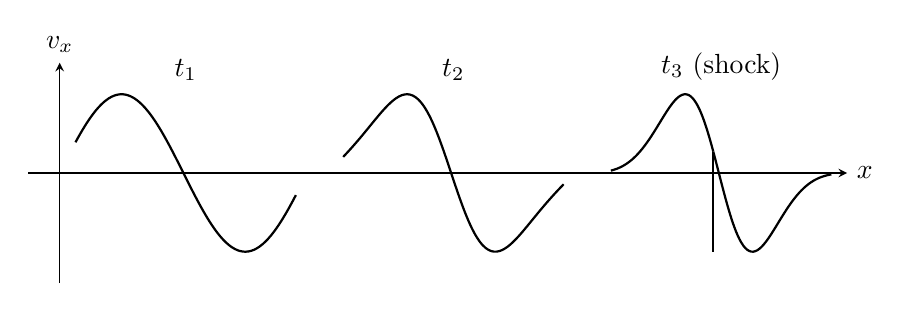
\begin{tikzpicture}[>=stealth, scale=1.0]
  \draw[->] (-0.4,0) -- (10,0) node[right] {$x$};
  \draw[->] (0,-1.4) -- (0,1.4) node[above] {$v_x$};
  % t1: clean sine
  \draw[thick,domain=0.2:3.0,smooth,samples=80] plot (\x, {sin(deg(2*\x))});
  \node[above] at (1.6,1.05) {$t_1$};
  % t2: leaning sawtooth (skewed)
  \begin{scope}[xshift=3.4cm]
    \draw[thick,domain=0.2:3.0,smooth,samples=80] plot (\x, {sin(deg(2*\x - 0.5*sin(deg(2*\x))))});
    \node[above] at (1.6,1.05) {$t_2$};
  \end{scope}
  % t3: vertical front
  \begin{scope}[xshift=6.8cm]
    \draw[thick,domain=0.2:1.5,smooth,samples=60] plot (\x, {sin(deg(2*\x - 0.95*sin(deg(2*\x))))});
    \draw[thick] (1.5,{sin(deg(2*1.5 - 0.95*sin(deg(2*1.5))))}) -- (1.5,-1.0);
    \draw[thick,domain=1.5:3.0,smooth,samples=60] plot (\x, {sin(deg(2*\x - 0.95*sin(deg(2*\x))))});
    \node[above] at (1.6,1.05) {$t_3$ (shock)};
  \end{scope}
\end{tikzpicture}
\end{center}

Estimate the breaking time. Two neighbouring characteristics carrying $v_x$ and $v_x+\Delta v_x$, initially separated by $\Delta x$, converge at relative speed $|\Delta v_x|$:
\[ \tau \sim \frac{\Delta x}{|\Delta v_x|}. \]
Write $\Delta v_x \sim \Delta x\,\partial_x v_x$ at the steepest descent of $v_x(x,0)=v_0\sin(kx)$:
\[ \partial_x v_x\big|_\text{min} = -kv_0. \]
Take the magnitude:
\[ \tau_\text{break} \sim \frac{\Delta x}{|\partial_x v_x|\Delta x} = \frac{1}{kv_0}. \]
The implicit-solution analysis confirms the prefactor of unity:
\begin{equation}
\boxed{\;\tau_\text{break} = \frac{1}{kv_0}.\;}
\end{equation}

\end{document}
